\taskpic{ На непроводящий гладкий стержень, изогнутый под прямым
  углом, насажены две бусинки равных масс $m$, несущие заряды
  противоположных знаков $Q_1$ и $Q_2$. В начальный момент бусинки
  неподвижны и находятся на расстоянии $d$ и $2d$ от угла. Отпустим
  их. Где окажется дальняя бусинка, когда ближняя доедет до вершины
  угла?  } 
{
  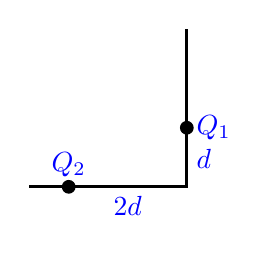
\begin{tikzpicture}
    \draw[very thick] (0,0) -- (2,0) -- (2,2);
    \draw[fill=black] (0.5,0) circle (0.08cm) node[above,blue] {$Q_2$};
    \draw[fill=black] (2,0.75) circle (0.08cm) node[right,blue]
    {$Q_1$};
    \draw (1.25,0) node [below,blue] {$2d$};
    \draw (2,0.35) node [right,blue] {$d$};
  \end{tikzpicture}
}
% Белорусские олимпиады, 1991, №2